\documentclass[UTF8]{ctexart}
\ctexset { section = { format={\Large \bfseries } } }
\pagestyle{plain}
\usepackage{float}
\usepackage{amsmath}
\usepackage{amssymb}
\usepackage{listings}
\usepackage{graphicx}
\usepackage{xcolor}
\usepackage{geometry}
\geometry{a4paper,scale=0.8}
\usepackage{caption}
\renewcommand{\abstractname}{\large Abstract}
\usepackage{booktabs}
\usepackage{siunitx}
\usepackage{hyperref}
\renewcommand{\refname}{References}
\captionsetup[figure]{name={Figure}}
\captionsetup[table]{name={Table}}

\lstset{
language=Python, % 设置语言
basicstyle=\ttfamily, % 设置字体族
breaklines=true, % 自动换行
keywordstyle=\bfseries\color{blue}, % 设置关键字为粗体,
morekeywords={}, % 设置更多的关键字,用逗号分隔
emph={self}, % 指定强调词,如果有多个,用逗号隔开
emphstyle=\bfseries\color{Rhodamine}, % 强调词样式设置
commentstyle=\color{black!50!white}, % 设置注释样式,斜体,浅灰色
stringstyle=\bfseries\color{red!90!black}, % 设置字符串样式
columns=flexible,
numbers=left, % 显示行号在左边
numbersep=2em, % 设置行号的具体位置
numberstyle=\footnotesize, % 缩小行号
frame=single, % 边框
framesep=1em % 设置代码与边框的距离
}

\title{\textbf{Data Structure Project1}\\{\Large Chinese-English Dictionary based on Binary
Search Tree}}

\author{吴嘉骜 21307130203}
\date{\today}

\begin{document}

\maketitle
\begin{abstract}
    \normalsize
    \noindent
    This report presents the implementation of an English-Chinese dictionary using advanced tree data structures: Red-Black trees and B-trees. 
    We first introduce the significance and characteristics of these structures, setting the context for their application. 
    In the Implementation section, we provide a description on structures and procedures involved in the manipulation of Red-Black trees and B-trees. 
    We then move on to experiment and list the time cost of initializing, deletion and insertion operations from files, together with search operations.
    Additionally, we analysis the results and compare the two data structures. 
    A user-friendly interface is offered to ensure that end-users can easily navigate and utilize the system to its full potential. 
    Finally, we discuss the limitations encountered during implementation and propose possible directions for future enhancements and research.
\end{abstract}

\noindent
\textbf {Project Objective}\\  The objective of this project is to delve deeper 
into the understanding of advanced tree data structures, particularly focusing on Red-Black trees and B-trees,
by implementing a Chinese-English dictionary.\\
\noindent
\textbf {Experiment environment} \\
    Windows 11 VsCode Python 3.11.5 64-bit

\section{Introduction}
\setlength{\parindent}{0pt}
Data structures play a crucial role in computer science, significantly impacting the 
efficiency and performance of algorithms and applications. 
Among these, tree structures such as \textbf{Red-Black trees} and \textbf{B-trees} stand out due to their 
ability to maintain balanced states, ensuring optimized operations even in the worst-case scenarios. It 
is of importance to understand the theoretical foundations of these structures, as well as their
practical applications, in order to harness their full potential.

\subsection{Red-Black Trees}
Red-Black trees are a type of self-balancing binary search tree, where every node 
contains an extra bit for denoting the color of the node, either red or black. 
This color coding is vital in ensuring a balanced structure, which in turn guarantees 
the tree's operations—such as search, insert, and delete—have a time complexity of $O(log n)$. 
The Red-Black tree maintains its balance by following specific properties and performing 
color changes and rotations during insertions and deletions.

\subsection{B-Trees}
B-trees, on the other hand, are balanced tree data structures optimized for systems 
that read and write large blocks of data, such as databases and file systems. 
They are particularly well-suited for storage systems since they can efficiently 
handle large amounts of data while maintaining a balanced structure. 
B-trees ensure all leaves are at the same level, and each node contains a certain number 
of keys sorted in a particular order. 
This characteristic guarantees fast search, insert, and delete operations, 
which are all performed in $O(log n)$ time.

\subsection{Project Task}
In this project, we focus on implementing an English-Chinese dictionary using Red-Black trees and B-trees respectively.
The tasks involve initializing both trees with specific input files, performing deletions 
and insertions, and ensuring correct search operations. 
Additionally, the project requires printing the tree in a preorder traversal 
to a text file, ensuring a clear and accurate representation of the tree`s structure.
It is renewcommanded to devise a user-friendly interface to allow end-users to interact with the dictionary.

\section{Implementation}
Most of the algorithms refer to \textit{Introduction to Algorithms} \cite{CLRS}, which are omitted here because they are too verbose and can be found in the textbook.
We will describe the structure of the main two \texttt{Python} scripts, as well as some noteworthy details in programming.

\subsection{Red-Black Trees}
The implementation of Red-Black trees is in \texttt{rb\_tree.py}.

\subsubsection*{Structure}
First, we define an \texttt{RBNode} class to represent a node in the Red-Black tree. Its attributes and 
typical functions are as follows:\\

\texttt{RED} and \texttt{BLACK} constants represent the color of the node.\\
\texttt{\_\_init\_\_}: Initializes a new node with $\textit{key, value, color, left child, right child}, and \textit{parent}$.\\
\texttt{is\_red}: Returns \texttt{True} if the node's color is red.\\
\texttt{is\_black}: Returns \texttt{True} if the node's color is black.\\
\texttt{set\_red}: Sets the node's color to red.\\
\texttt{set\_black}: Sets the node's color to black.\\
\texttt{\_\_str\_\_}: Provides a string representation of the node.\\

Then we come to the \texttt{RedBlackTree} class, which represents a Red-Black tree. Its attributes and main functions are
described as follows, where we omit the $\texttt{self}$ parameter for brevity:\\
\texttt{\_\_init\_\_}: Initializes an empty Red-Black Tree with a sentinel \texttt{nil} node, which is black with arbitrary key and value, representing a NULL leaf node.\\

\textbf{Search functions}:\\
\texttt{search(x, key)}: Searches for a node with the given key in the tree rooted at \texttt{x}.\\
\texttt{minrb(x)}: Finds the minimum node in the tree rooted at \texttt{x}.\\
\texttt{maxrb(x)}: Finds the maximum node in the tree rooted at \texttt{x}.\\
\texttt{successor(x)}: Finds the successor of node \texttt{x}.\\
\texttt{predecessor(x)}: Finds the predecessor of node \texttt{x}.\\
\texttt{rangesearch(low,high)}: Search for words in the specified range [low, high].\\
\texttt{singlesearch(en)}: Search for an English word in the tree.\\

\textbf{Rotations}:\\
These two auxiliary functions are used to maintain the Red-Black Tree properties after insertions and deletions.\\
\texttt{\_left\_rotate(x)}: Performs a left rotation on the subtree rooted at \texttt{x}.\\
\texttt{\_right\_rotate(y)}: Performs a right rotation on the subtree rooted at \texttt{y}.\\

\textbf{Insertion functions}:\\
The main insertion function is \texttt{insertrb(z)}, and the auxiliary function \texttt{\_insert\_fixup(z)} is used after
a node is inserted to fix up the possible violations of the Red-Black Tree properties.\\
\texttt{insertrb(z)}: Inserts a new node \texttt{z} into the tree.\\
\texttt{\_insert\_fixup(z)}: Fixes the Red-Black Tree properties after an insertion.\\
\texttt{insert\_word(en,cn)}: Insert an English word and its Chinese translation in the Red-Black Tree.\\

\textbf{Deletion functions}:\\
The main deletion function is \texttt{deleterb(z)}, the auxiliary function \texttt{\_transplant(u, v)} is for
a node replacement, and \texttt{\_delete\_fixup(x)} are used after a node is deleted to fix up the properties.\\
\texttt{deleterb(z)}: Deletes the node \texttt{z} from the tree.\\
\texttt{\_transplant(u,v)}: Replaces the subtree rooted at node \texttt{u} with the subtree rooted at node \texttt{v}.\\
\texttt{\_delete\_fixup(x)}: Fixes the Red-Black Tree properties after node \texttt{x} is actually deleted from the tree.\\
\texttt{delete\_word(en)}: Delete an English word and its Chinese translation from the Red-Black Tree.\\

\textbf{Printing and file operations}:\\
\texttt{preorder\_print}: Preorder prints the Red-Black Tree to a file or the console, with a specific format.\\
\texttt{initialize}: Initializes the Red-Black Tree with data from a file.\\
\texttt{batch\_op}: Performs batch operations of insertion/deletion from text files on the Red-Black Tree.\\

\subsubsection*{Details}
To ensure that there are no duplicate insertions, we examine the return values of the functions related to insertion. During each recursive search for the position of a key (i.e., the subtree where it should be placed), we check whether the value equals that of an existing node. If a match is found, a value of \texttt{False} is returned, which propagates up through the recursion stack. This mechanism ensures that a single downward search suffices to either insert the key or confirm that insertion is not feasible. 

For deletion, avoiding the removal of non-existent nodes is somewhat more complex compared to insertion. Our approach entails an initial search to confirm the presence of the node. If the node is found, deletion proceeds; otherwise, it is aborted. While this procedure incurs an additional cost due to the extra search, it allows us to circumvent the complexities of deletion when the node is confirmed to be absent.

\subsection{B-Trees}
The implementation of B-trees is in \texttt{b\_tree.py}.

\subsubsection*{Structure}
First, we define a \texttt{BTNode} class to represent a node in the B-tree. Its attributes and typical functions are as follows:\\

\texttt{\_\_init\_\_}: Initializes a new node with $\textit{n, keys, values, isleaf,}$ and $\textit{c}$.\\
\texttt{n}: Represents the number of keys currently stored in the node.\\
\texttt{keys}: A list of keys (English words) stored in the node, arranged in ascending order.\\
\texttt{values}: A list of values (Chinese translations) stored in the node, corresponding to the keys.\\
\texttt{isleaf}: A boolean value indicating whether the node is a leaf. The default value is True.\\
\texttt{c}: A list of pointers to child nodes.\\
\texttt{is\_full}: Checks if the node is full based on the order of the B-tree and returns a boolean value.\\

Then we come to the \texttt{BTree} class, which represents a B-tree. Its attributes and main functions are described as follows, where we omit the $\texttt{self}$ parameter for brevity:\\
\texttt{\_\_init\_\_}: Initializes a B-tree with a specified order, \texttt{t}, and creates an empty root node.\\

\textbf{Search functions}:\\
\texttt{search(key, x)}: Searches for a node with the given key in the tree rooted at node \texttt{x}.\\
\texttt{singlesearch(en)}: Searches for a given English word in the tree and returns the Chinese translation if found.\\
\texttt{rangesearch(low,high)}: Searches for words in a specified range \texttt{[low, high]} and returns a list of tuples containing the words and their meanings.\\

\textbf{Insertion functions}:\\
The main insertion function is \texttt{insertb(z)}, and \texttt{\_insert\_nonfull(x, k, v)} and \texttt{\_split\_child(x, i)} are auxiliary functions.\\
\texttt{insertb(key, value)}: Inserts a given key and its value into the B-tree.\\
\texttt{\_insert\_nonfull(x, key, value)}: Inserts a given key and its value into a non-full node.\\
\texttt{\_split\_child(x)}: Splits a full child node of a given node.\\
\texttt{\_split\_root}: Splits the root of the tree if it becomes full post-insertion.\\
\texttt{insert\_word(en, cn)}: Inserts a given English word and its Chinese translation into the B-tree.\\

\textbf{Deletion functions}:\\
The main deletion function is \texttt{deleteb(z)}, the rest are auxiliary functions except \texttt{deleteword}.\\
\texttt{deleteb(key,x)}: Deletes a given key from the tree rooted at node \texttt{x}.\\
\texttt{\_delete\_internal\_node(x,key)}: Deletes a given key from an internal node.\\
\texttt{\_delete\_predecessor(x)}: Deletes the predecessor of a given key.\\
\texttt{\_delete\_successor(x)}: Deletes the successor of a given key.\\
\texttt{\_delete\_merge(x,i,j)}: Merges a key and one of its two neighboring child nodes.\\
\texttt{\_delete\_sibling(x,i,j)}: Borrows a key from a sibling node.\\
\texttt{delete\_word(en)}: Deletes a given English word from the B-tree.\\

\textbf{Printing and file operations}:\\
\texttt{preorder\_print}: Preorder prints the B-tree to a file or the console.\\
\texttt{initialize}: Initializes the B-tree with data from a specified file.\\
\texttt{batch\_op}: Performs batch operations of insertion/deletion from a specified text file on the B-tree.\\

\subsubsection*{Details}
The strategies to avoid duplicate insertions and the deletion of non-existent nodes in B-tree (BT) are consistent with those employed in the Red-Black Tree (RBT). Just like in RBT, before an insertion or deletion operation, a search is performed to check the existence or absence of the node in question, thereby ensuring that only valid nodes are inserted or deleted from the tree, minimizing the chances of erroneous operations.

As the pseudocode for deletion is not available in the textbook, I struggle to implement it with efforts to ensure that the tree remains balanced after the operation.
There are some details that need to be paid attention to, as I got confused for some moment during my own work:\\
First and foremost, we have to guarantee that the node on which a resursion is performed has at least $t$ keys, which is 1 plus the minimum number of keys in a non-root node.
When searching down the tree, we have to take care of the child node with underfull keys, and we have to merge or borrow keys from its sibling node if necessary.\\
For Case2a and Case2b, we need to find the predecessor or successor in the subtree, which is the leftmost or rightmost node of it.
The point is that once we have chosen a target, we have to pass down in a fixed direction, and no longer consider again finding predecessors or successors.
The resursion also requires that the node on which it is performed have at least $t$ keys, so a merge or borrow operation may also be needed.\\
For Case2c and Case3b, we are encountered with merge or borrow operations, making indices out of range a common problem. One special situation is that if parent node is the root, it could end up having no keys.
In this case, we have to delete the root and set its child node as the new root, and change the resursion accordingly.\\

\section{Results and Analysis}
We test our codes both on single operations and batch operations, according to the requirements of the project.\\
1. Insert into trees the data in the file 1\_initial.txt. The results are saved to rbt\_1.txt and bt\_1.txt.\\
2. Delete the data in the file 2\_delete.txt. The results are saved to rbt\_2.txt and bt\_2.txt.\\
3. Add the data in the file 3\_insert.txt. The results are saved to rbt\_3.txt and bt\_3.txt.\\
4. Query a word.\\
5. Query some words.\\
For the first three steps, the whole time cost results are saved to timecost.txt, and we only show the average time cost of each operation in the following table.\\
\begin{table}[h]
    \centering
    \caption{Average time for different operations in RBT and BT ($10^{-5}$s)}
    \label{tab:times}
    \begin{tabular}{lccc}
    \toprule
        & \textbf{Initialization} & \textbf{Deletion} & \textbf{Insertion} \\
    \midrule
    \textbf{RBT} & \num{5.437} & \num{9.954} & \num{9.623} \\
    \textbf{BT} & \num{4.527} & \num{9.847} & \num{9.153} \\
    \bottomrule
    \end{tabular}
    \end{table}

We plot the result in a bar chart, as shown in Figure 1.\\
\begin{figure}[h]
    \centering
    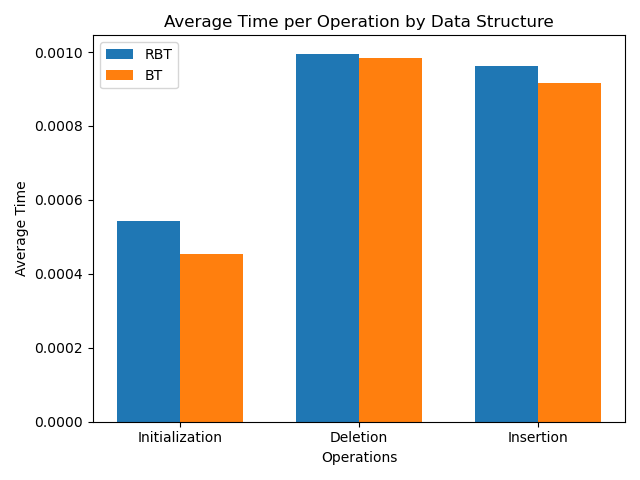
\includegraphics[width=0.6\textwidth]{Figure_1.png}
    \caption{Average time for different operations in RBT and BT ($10^{-5}$s)}
    \label{fig:times}
\end{figure}
\newpage
For the last two steps, the results are undoubtedly the same. We exhibit a query example here.\\
\begin{lstlisting}
    # Single word query
    meaning = bt.singlesearch('cybernetic')
    print(f'{meaning}')

    # Output
    控制论的

    # Range query
    result = bt.rangesearch('cuculliform', 'culmination')
    for word, meaning in result:
        print(f'{word}: {meaning}')

    # Output
    cuculliform: 兜帽状的
    cucumiform: 黄瓜状的
    cuddle: 拥抱
    cuffy: 黑人
    culicid: 蚊科的
    culicine: 库蚊的
    cull: 精选
    cullet: 碎玻璃
    culminate: 达到顶点
    culmination: 顶点
\end{lstlisting}

\textbf{Analysis}:\\
From the time record, we can see that both trees present a very small time requirement for the three operations, 
which is a good indication of efficiency. The times are very close to each other, probably due to our limited data size.\\
However, the B-tree consistently shows lesser time across all operations, probably because the branching factor of the B-tree contributes to its efficiency. 
A larger branching factor can lead to a more shallow tree, potentially reducing the number of steps required to perform insertions, deletions, and searches.\\
Furthermore, the B-tree's structure can lead to faster disk access times when dealing with disk storage, even though in our case the operations were performed in memory.\\
In conclusion, while both data structures show strong performance and are well-suited for different use cases, the B-tree demonstrated a slight edge in terms of efficiency in our tests.
However, if the difference in time is negligible, then the choice between RBT and BT might come down to other factors such as ease of implementation, memory usage, or specific use case requirements.\\

\section{Interface and Usage}
The interface picture is shown in Figure 2.\\
\begin{figure}[h]
    \centering
    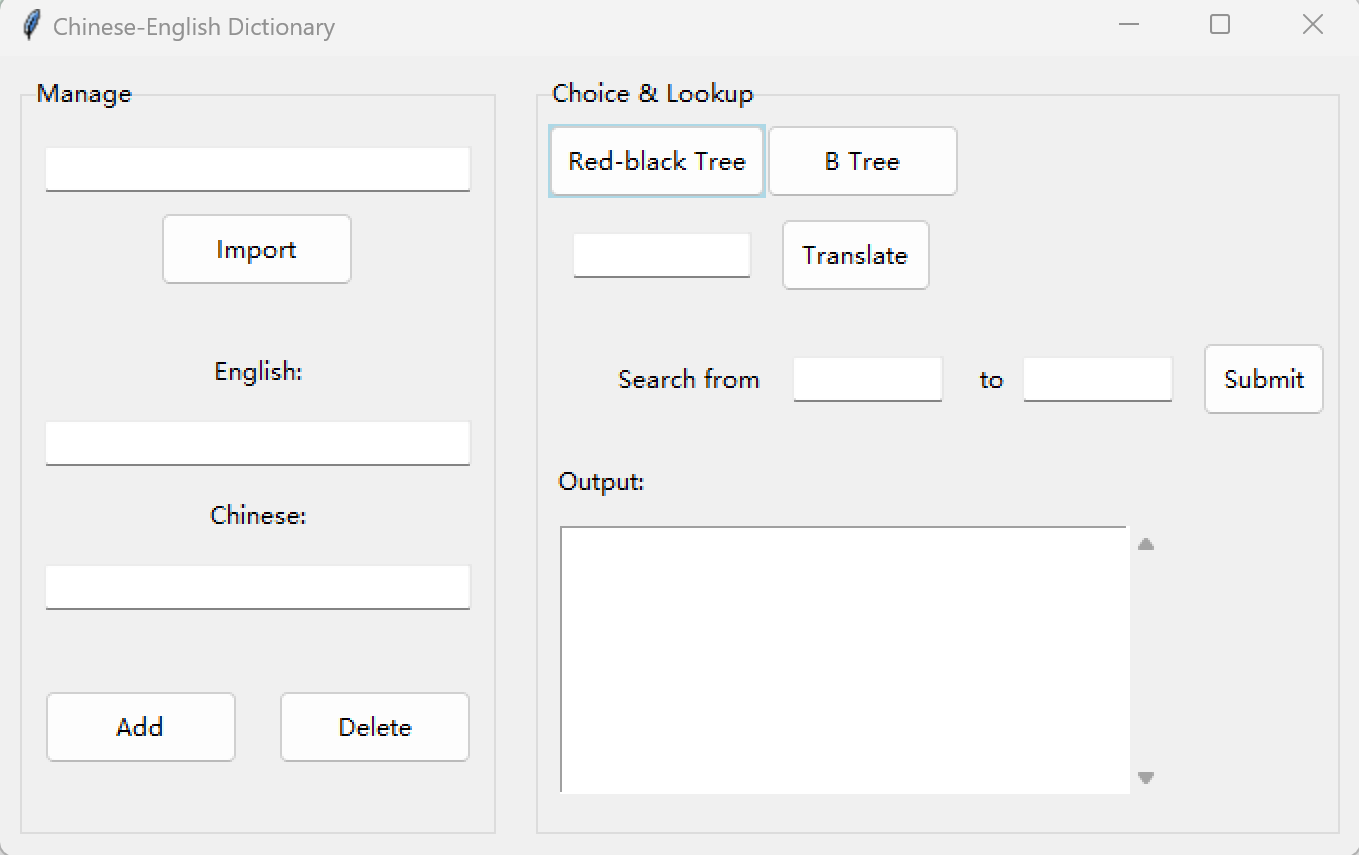
\includegraphics[width=0.7\textwidth]{UI.png}
    \caption{Interface}
    \label{fig:interface}
\end{figure}

As is shown in the picture, the interface is quite simple and easy to use.\\
The left part is designed for a user to import a file to initialize the dictionary, or to
add or delete a single word from the dictionary. For insertion, both English and Chinese words are needed; 
for deletion, only the English word is needed.\\
The right-top part is a button to choose which kind of tree to use, and the right-bottom part is for look-up.
For a single word query, it gives the corresponding Chinese translation if the word is in the dictionary;
for a range query, it gives a list of words and their meanings in the specified range.\\

\section{Discussion}

\subsection{Limitations}
The current implementation of the English-Chinese dictionary has several limitations that could be addressed in future work:

1. \textbf{Disk Utilization:} Despite the B-tree being a data structure that is well-suited for disk storage, in the current implementation, operations are carried out in memory, which does not leverage the potential for efficient disk access and storage. The inherent design of B-trees to minimize disk I/O operations has not been fully utilized, thus possibly affecting the performance when handling large datasets.

2. \textbf{User Interface Design:} The User Interface (UI) design is quite plain, which could affect the ease of use and the overall user experience.

3. \textbf{Code Reusability:} The code is not highly reusable. While it serves the purpose of implementing an English-Chinese dictionary efficiently, adapting the code for other applications or data types may require significant modifications.

\subsection{Future Work}
Going forward, there are several improvements that can be considered to enhance the functionality and applicability of the project:

1. \textbf{Satellite Data Storage:} The application can be extended to handle satellite data storage, which often requires efficient indexing and retrieval mechanisms. The structure of B-trees could be utilized to build robust indexing systems to manage and query satellite data effectively.

2. \textbf{Utilizing B+ Trees:} Transitioning to a B+ tree structure could be explored for future implementations. B+ trees have some advantages over B-trees, including more efficient range querying and better utilization of disk space due to the linked leaves.

3. \textbf{Disk-Based Operations:} Modifying the implementation to perform disk-based operations could significantly improve the performance of the application, especially when dealing with large datasets. This would align with the inherent design of B-trees for disk storage and access.

4. \textbf{Enhanced User Interface:} Improving the User Interface to be more intuitive and user-friendly can enhance the usability of the application.

In conclusion, we have implemented main functions of Red-Black trees and B-trees successfully despite some struggles in the process. We applied these two data structures to build
an English-Chinese dictionary, and we have also provided an interface for users to use the dictionary. The experiment result 

\begin{thebibliography}{9}
\bibitem{CLRS}
Cormen, T. H., Leiserson, C. E., Rivest, R. L., Stein, C. (2022). 
\textit{Introduction to Algorithms} (4th ed.). The MIT Press.
\end{thebibliography}

\end{document}